\chapter{QUALITY MANAGEMENT}

\renewcommand{\headrulewidth}{0.5pt}
\renewcommand{\footrulewidth}{0.5pt}
\thispagestyle{plain}
\pagestyle{fancy}
\fancyhf{}
\fancyhead[L]{\textbf{CHAPTER 3}}
\fancyhead[R]{\textbf{Graduate Report}}
\raggedright
\fancyfoot[L]{From: Nguyen Van Anh Tuan}
\fancyfoot[R]{Page \thepage}

\justifying

\section{Simulator Maintenance}
    Reports-based database is primarily designed as a means to reporting simulator maintenance, organize quality logs and analyze 
    performance measures that can be monitored against objectives. Such measures often referred to as Metrics, will be reviewed by 
    the Certifying Authority as part of its oversight of the Quality System, at least, annual basis as well as an itegral part of 
    the Quality Audit process.
    \subsection{Scheduled Maintenance}
        The maintenance procedures for the simulator will be in accordance with the manufacturer supplied maintenance documentation 
        and local procedures. The routine maintenance requirement is grouped into the following categories.
        \begin{itemize}
            \item Hourly routine Maintenance
            \item Daily Routine Maintenance
            \item Weekly Routine Maintenance
            \item Bi-weeky Routine Maintenance
            \item Monthly Routine Maintenance
            \item Quarterly Routine Maintenance
            \item Six Monthly Routine Maintenance
            \item Annually Routine Maintenance
            \item Five-yearly Routine Maintenance
        \end{itemize}
        The numbers of categories applied for each FSTD (Flight Simulation Training Devices) depend on the official maintenance manual 
        issued by FSTD manufacture. \\ 
        \vspace{3mm}
        Based on "Meantime Between Failure" MBF analysis, should a maintenance procedure require to be performed more frequently than the 
        manufacturer recommends its category shall be changed accordingly. \\ 
        \vspace{3mm}
        Each Routine Maintenance tasks will be scheduled by the "Simulator Schedule Calendar" for each simulator. For specific Scheduled 
        Maintenance actions are described in detail as follow:
        \begin{itemize}
            \item \textbf{Daily Routine Maintenance}
            \begin{itemize}
                \item Computers and Peripherals: Inspect and test the motion system
                \item Motion: Inspect and test the motion system
                \item Smoke Generation: Check fluid level
                \item Visual: Perform and image evalution
            \end{itemize}
            \item \textbf{Weekly Routine Maintenance}
            \begin{itemize}
                \item Smoke Generation: Drain fluid 
                \item Visual: Geometry, Full calibration, Night luminance
            \end{itemize}
            \item \textbf{Monthly Routine Maintenance}
            \begin{itemize}
                \item Air Conditioning and Equipment Cooling: Inspect the flexible hose between the air conditioner and flight compartment; 
                Inspect the air conditioner intake filter; Inspect water drain, hoses and fittings
                \item Crew Accessway: Inspect flight compartment access gate
                \item Electrical: Perform UPS battery test; Electromagnetic Compatibility (EMC) maintenance check of electronic enclosure doors; 
                Test the operation of the entrance emergency lighting
                \item Motion: Clean the motion actuators and the outside of the motion control cabinet; Test the Emergency Power Off (EPO) circuit
                \item Visual: Clean the air filters on IG PCs
            \end{itemize}
            \item \textbf{Three-Month Routine Maintenance}
            \begin{itemize}
                \item Air Conditioning and Equipment Cooling: Perform a functional check of the airflow and temperature monitoring system
                \item Motion: Lubricate the upper and lower bearings; Test the interlock circuit; Test the drawbridge limit switches; Inspect 
                the motion control cabinet and electrical cabling; Perform disk maintenance on the real time controller computer
            \end{itemize}
            \item \textbf{Six-Month Routine Maintenance}
            \begin{itemize}
                \item Crew Accessway: Test the safety interlock and STOP button
                \item Electrical: Grounding inspection
                \item Motion: Lubricate motion actuators
                \item Visual: Golden Alignment
            \end{itemize}
            \item \textbf{Annually Routine Maintenance}
            \begin{itemize}
                \item Computer and Peripherals: Computer cleaning
                \item Crew Accessway: Inspect the Interference Relay
                \item Electrical: Test the battery of the entrance emergency light panel
                \item Motion: Inspect and check-tighten the motion system bolts to specified torque; Motion system vibration isolator inspection; 
                Inspect the platform structure welds; Check-tighten the bolts securing the fligh compartment tie-beams; Replace the air filters 
                on the motion control cabinet; Clean the inside of the motion control cabinet
                \item Safety: Test the motion and control loading (C/L) cutoff switches; Test the motion inhibit switches
                \item Smoke Generation: Inspect and change filter in the filter/fan smoke extraction assembly
            \end{itemize}
            \item \textbf{Five-Year Routine Maintenance}
            \begin{itemize}
                \item Electrical: Replace the emergency lighting battery in the celing light controller
            \end{itemize}
        \end{itemize} 
        Monthly, Six-Monthly and Yearly Maintenance are formally scheduled as programmed maintenance slots. \\
        \vspace{3mm}
        The FSTD Technical Support engineer shall be responsible for ensuring that Maintenance Procedures are carried out at the recommended time 
        interval and the correct procedure is adhered to. \\
        \vspace{3mm}
        Every scheduled maintenance form must be filled and signed by FSTD Technical Support engineer in proper manner when appropriate scheduled 
        maintenance is done. \\ 
        \vspace{3mm}
        Scheduled maintenance Logs have column where is checkboxes YES/NO to indicate if planned action was performed. If action was not performed and 
        indicated as "NO", then comment should be written and specific action number should be indicated. \\ 
        \vspace{3mm}
        The signed "Maintenance Scheduling Logs" must be put into "Maintenance Scheduling Logs" folder on a monthly basis. \\ 
        \vspace{3mm}
        If, as a result of any maintenance, remedial action is required a comment should be written at appropriated field of actual scheduled maintenance 
        log and "Technical Defects Log" shall be raised, to reflect the work required/performed, stating any parts used. If necessary, maybe filled up or 
        updated any other reprorts.
    \subsection{Unschedule Maintenance}
        \subsubsection{Defect Reporting System}
            Each observed technical defect must be listed using \textbf{Form 27 "Notice to instructor"} \\ 
            \vspace{3mm}
            In this document provides the information for instructor about actual open defects on simulator, inaccuracies or anything else that could 
            confuse instructor to use simulator in proper manner. There are not provided defects which have no effect on training. Notices to instructor 
            should be updated in accordance with any resolved problem or in the case if a new problem is observed. \\
            \vspace{3mm}
            FSTD Technical Support engineer should ensure that notice to instructor is updated by actual situation. \\ 
            \vspace{3mm}
            Notice to instructor is placed for public access on the way to appropriate simulators to inform instructors about open defects. Duty engineer 
            should explain notices in more details to instructor if required. \\
            \vspace{3mm}
            Form 27 should be filled using the following guidance:
            \begin{enumerate}
                \item \textbf{"Category"} - defect category;
                \item \textbf{"SubCategory"} - defect subcategory;
                \item \textbf{Description"} - notice text. It means description of raised problem and/or recommended actions how instructor should react 
                to this problem
            \end{enumerate}
            "Technical Defect Log" - reference to appropriate Technical Defect Log for more information if required.
        \subsubsection{Defect Rectification Process}
            Every raised technical defect is named like "Open defect" until it will be resolved. Each technical defect shall be assigned "Effect on Training" 
            grade which means how much effect defect is providing for training session. Effect on training grade can be:
            \begin{itemize}
                \item \textbf{Level A} - The defect has a major impact on a training curriculum. The customer cannot perform the intended or planned training without 
                bringing negative effect training to the crew and no workaround can be found. The defect may jeopardize safe operation or maintenance of the 
                simulator. 
                \item \textbf{Level B} - The defect has a major impact on one or more areas of the training curriculum. Training can be partially conducted in these 
                areas but requires undesirable work-around procedures to be followed by the instructor/operator, or by the studen crew. The defect may have 
                a significant impact on maintenance procedures such that regular procedures cannot be followed or executed properly. 
                \item \textbf{Level C} - The defect has a minor impact on one or more areas of the training curriculum. Training task can be completed with or without 
                work around but one aspect of the task is incomplete or inaccurate. Or the defect has a minor impact on maintenance of the simulator or is 
                related to training aides (Training Aides: IOS MAP, Lesson Plan Editor, Brief-Debrief station, etc).
                \item \textbf{Level D} - Captured problems to be resolved relating to maintenance, documentation.
            \end{itemize}
            FSTD Technical Support engineer assigns Effect on training grade. He can discuss impact severity with FSTD Technical Support flight instructor if 
            needed. \\
            \vspace{3mm}
            If an "Open" technical defect has no direct effect on the training, but is deemed still to be an issue then it shall be treated as an "Open" fault 
            with the fault history being updated and its "Status" be reassigned accordingly. \\ 
            \vspace{3mm}
            If an "Open" technical defect has a direct effect on the training, which have no immediate solution, it shall be reassigned as an "Acceptable 
            Deferred Defect" (ADD). Should the ADD be investigated and it deemed that no immediate solution is being sought or available, the fault history 
            should be updated and its "Status" should be assigned as "Deferred". \\ 
            \vspace{3mm}
            Should an ADD be investigated and it deemed a solution is available, the fault history should be updated and its "Status" be reassigned accordingly. \\ 
            \vspace{3mm}
            ADD list should be provided for instructor before very training session in "Notice to Instructor" journal. F/O side slip ball indicator is stuck. \\ 
            \vspace{3mm}
            If effect grade is "Level A" then training sessions should be cancelled and moved to another time until defect will be fixed. If critical defect occurred 
            then Accountable Manager and Safety and Quality Assurance Manager should be informed immediately by email. Typically, there should be written Technical 
            Defect No. for reference and brief defect description. \\
            \vspace{3mm}
            As a result a technical defect is generated, it's "Category" assigned with defect feature. "Category" should represent general defect scope. \\ 
            \vspace{3mm}
            Defect "Sub Category" should be assigned with its sub feature if necessary. "Sub Category" represents defects scope under specified "Category". \\ 
            \vspace{3mm}
            The technical defect is to be investigated with the fault history being updated and its "Status" be reassigned accordingly. There are few "Status" 
            positions used: 
            \begin{itemize}
                \item \textbf{"Investigating"} - description of defect investigation progress;
                \item \textbf{"Deferred"} - defect status is "Acceptable Deferred Defect";
                \item \textbf{"Part Required"} - spare part required for repair progress but none is available. Spare part number (p/n) should be written;
                \item \textbf{"Part Ordered"} - required spare part is ordered and waiting for delivery. Order details or appropriate reference should be written;
                \item \textbf{"Part Received"} - ordered spare part received but there is no possibility to fit (simulator is in use, not enough manpower etc.);
                \item \textbf{"Other"} - any other action which can't be included under any of provided group;
                \item \textbf{"Resolved"} - defect is resolved;
                \item \textbf{"Expired"} - defect is no longer available
            \end{itemize}
            Each step in technical defect investigation progress should have written date, start time, finish time and duration. All these data will be used 
            for quality metrics. There should be written engineer name for each step of defect investigation. \\ 
            \vspace{3mm}
            There is general sequence of engineer actions:
            \begin{itemize}
                \item Technical defect observed;
                \item Raise appropriate technical defect report
            \end{itemize}
            Investigate technical defect and accordingly fill up technical defect report until defect will be resolved. Change defect report status accordingly 
            to actual defect investigation status.

\section{Parts Management}
    \subsection{Spare Parts Management}
        Spare parts are placed in the storage room. \\ 
        \vspace{3mm}
        FSTD Technical Support engineers can access spare parts at any time. The usage of spare parts must be traced using \textbf{Form 18 "Spare Part Log"}. 
        The quantity of available spare parts must be updated at the appropriate \textbf{Spare Parts Log}. \\
        \vspace{3mm}
        Form 18 includes:
        \begin{enumerate}
            \item \textbf{"Component name"} - the name of spare part;
            \item \textbf{"Part No."} - the part number of appropriate component;
            \item \textbf{"Serial No."} - the serial number of appropriate component;
            \item \textbf{"Qty."} - quantity of specific spare parts;
            \item \textbf{"Status"} - there should be described current status of specific spare part: Available, On maintenance, Not available, Need to order etc.;
            \item \textbf{"Location"} - brief description where to find that spare part;
            \item \textbf{"Comment"} - additional information about spare part.
        \end{enumerate}
        Simulator "Spare Parts Log" helps to manage usage of spare parts. "Spare Parts Logs" are put into "Spare Parts Logs" folder. \\ 
        \vspace{3mm}
        If the procedure of spare part exceeds the responsibility limits of FSTD Technical Support engineer, then Accountable Manager will be informed about required 
        spare part in 24 hours to get confirmation about further actions.

    \subsection{Component Removal - Installation}
        Simulator maintenance manual procedures must be adhered to when work is being carried out on the simulator. Conductive plastic wrist strap and a suitable lead 
        must be worn before handling any static sensitive devices. \\
        \vspace{3mm}
        Details of all work carried out, all components removed from or installed onto the simulator shall be recorded in the "Technical Defects Log". A summary of work 
        carried out is to be enterd in the relevant "Technical Defects Log". \\
        \vspace{3mm}
        Additional information to identify the removed or installed component, the location where it is placed shall be filled in the \textbf{Error! Reference source not 
        found}. All "Component Removal - Installation Logs" are put into "Component Removal - Installation Logs" folder on a monthly basis and sorted by date. \\
        \vspace{3mm}
        \textbf{Error! Reference source not found} contains:
        \begin{enumerate}
            \item \textbf{"Date/Time"} - time mark when job was done;
            \item \textbf{"Defect No."} - the number of appropriate Technical Defect Log;
            \item \textbf{"Destination Device Name"} - exact name, part and serial numbers (if available) of destination device where appropriate component was 
            installed or it is dedicated to install to;
            \item \textbf{"Component Name"} - the name of installed component;
            \item \textbf{"Component Specification"} - manufacturer's specifications of installed or removed component;
            \item Part No.;
            \item serial No.;
            \item other details (there can be written any other detail according to installed or removed component");
            \item \textbf{"Action"} - there should be selected the kind of job: Removal or Installation;
            \item \textbf{"Component Location"} - actual location of removed or installed component.
        \end{enumerate}

    \subsection{Repairable Components}
        All components, which have been repaired at an outstation, shall, upon receipt, be installed into the appropriate FSTD for functional and operational checks before 
        warranty period expires. Only then shall these repaired components be credited back to stores. The progress for all repaired components is documented by 
        \textbf{Form 17 "Repaired Component Log"}:
        \begin{enumerate}
            \item \textbf{"Date/Time"} - time mark when job was done;
            \item \textbf{"Defect No."} - the number of appropriate Technical Defect Log;
            \item \textbf{"Destination Device Name"} - exact name, part and serial numbers (if available) of destination device where appropriate component should be installed;
            \item \textbf{"Component name"} - the name of repaired component;
            \item \textbf{"Component specification"} - manufacturer's specifications of repaired component:
                \begin{itemize}
                    \item part No.;
                    \item serial No.;
                    \item other details (there can be written any other detail according to repaired component);
                \end{itemize}
            \item \textbf{"Company name"} - manufacture Company name of unserviceable component of name of potential repair company where to send unserviceable part;
            \item \textbf{"Additional information about company"} - there should be written any additional information related to service/manufacture company;
            \item \textbf{"Comment"} - any comments about unserviceable component.
        \end{enumerate}
        "Repaired Components Logs" are put into "Repaired Components Logs" folder on a monthly basis.

    \subsection{Unserviceable Components}
        All serviceable components removed from simulator shoud have an Unserviceable Component label attached with all relavant information to identify the component and the 
        particular technical defects log copy.
        \begin{figure}[H]
            \centering
            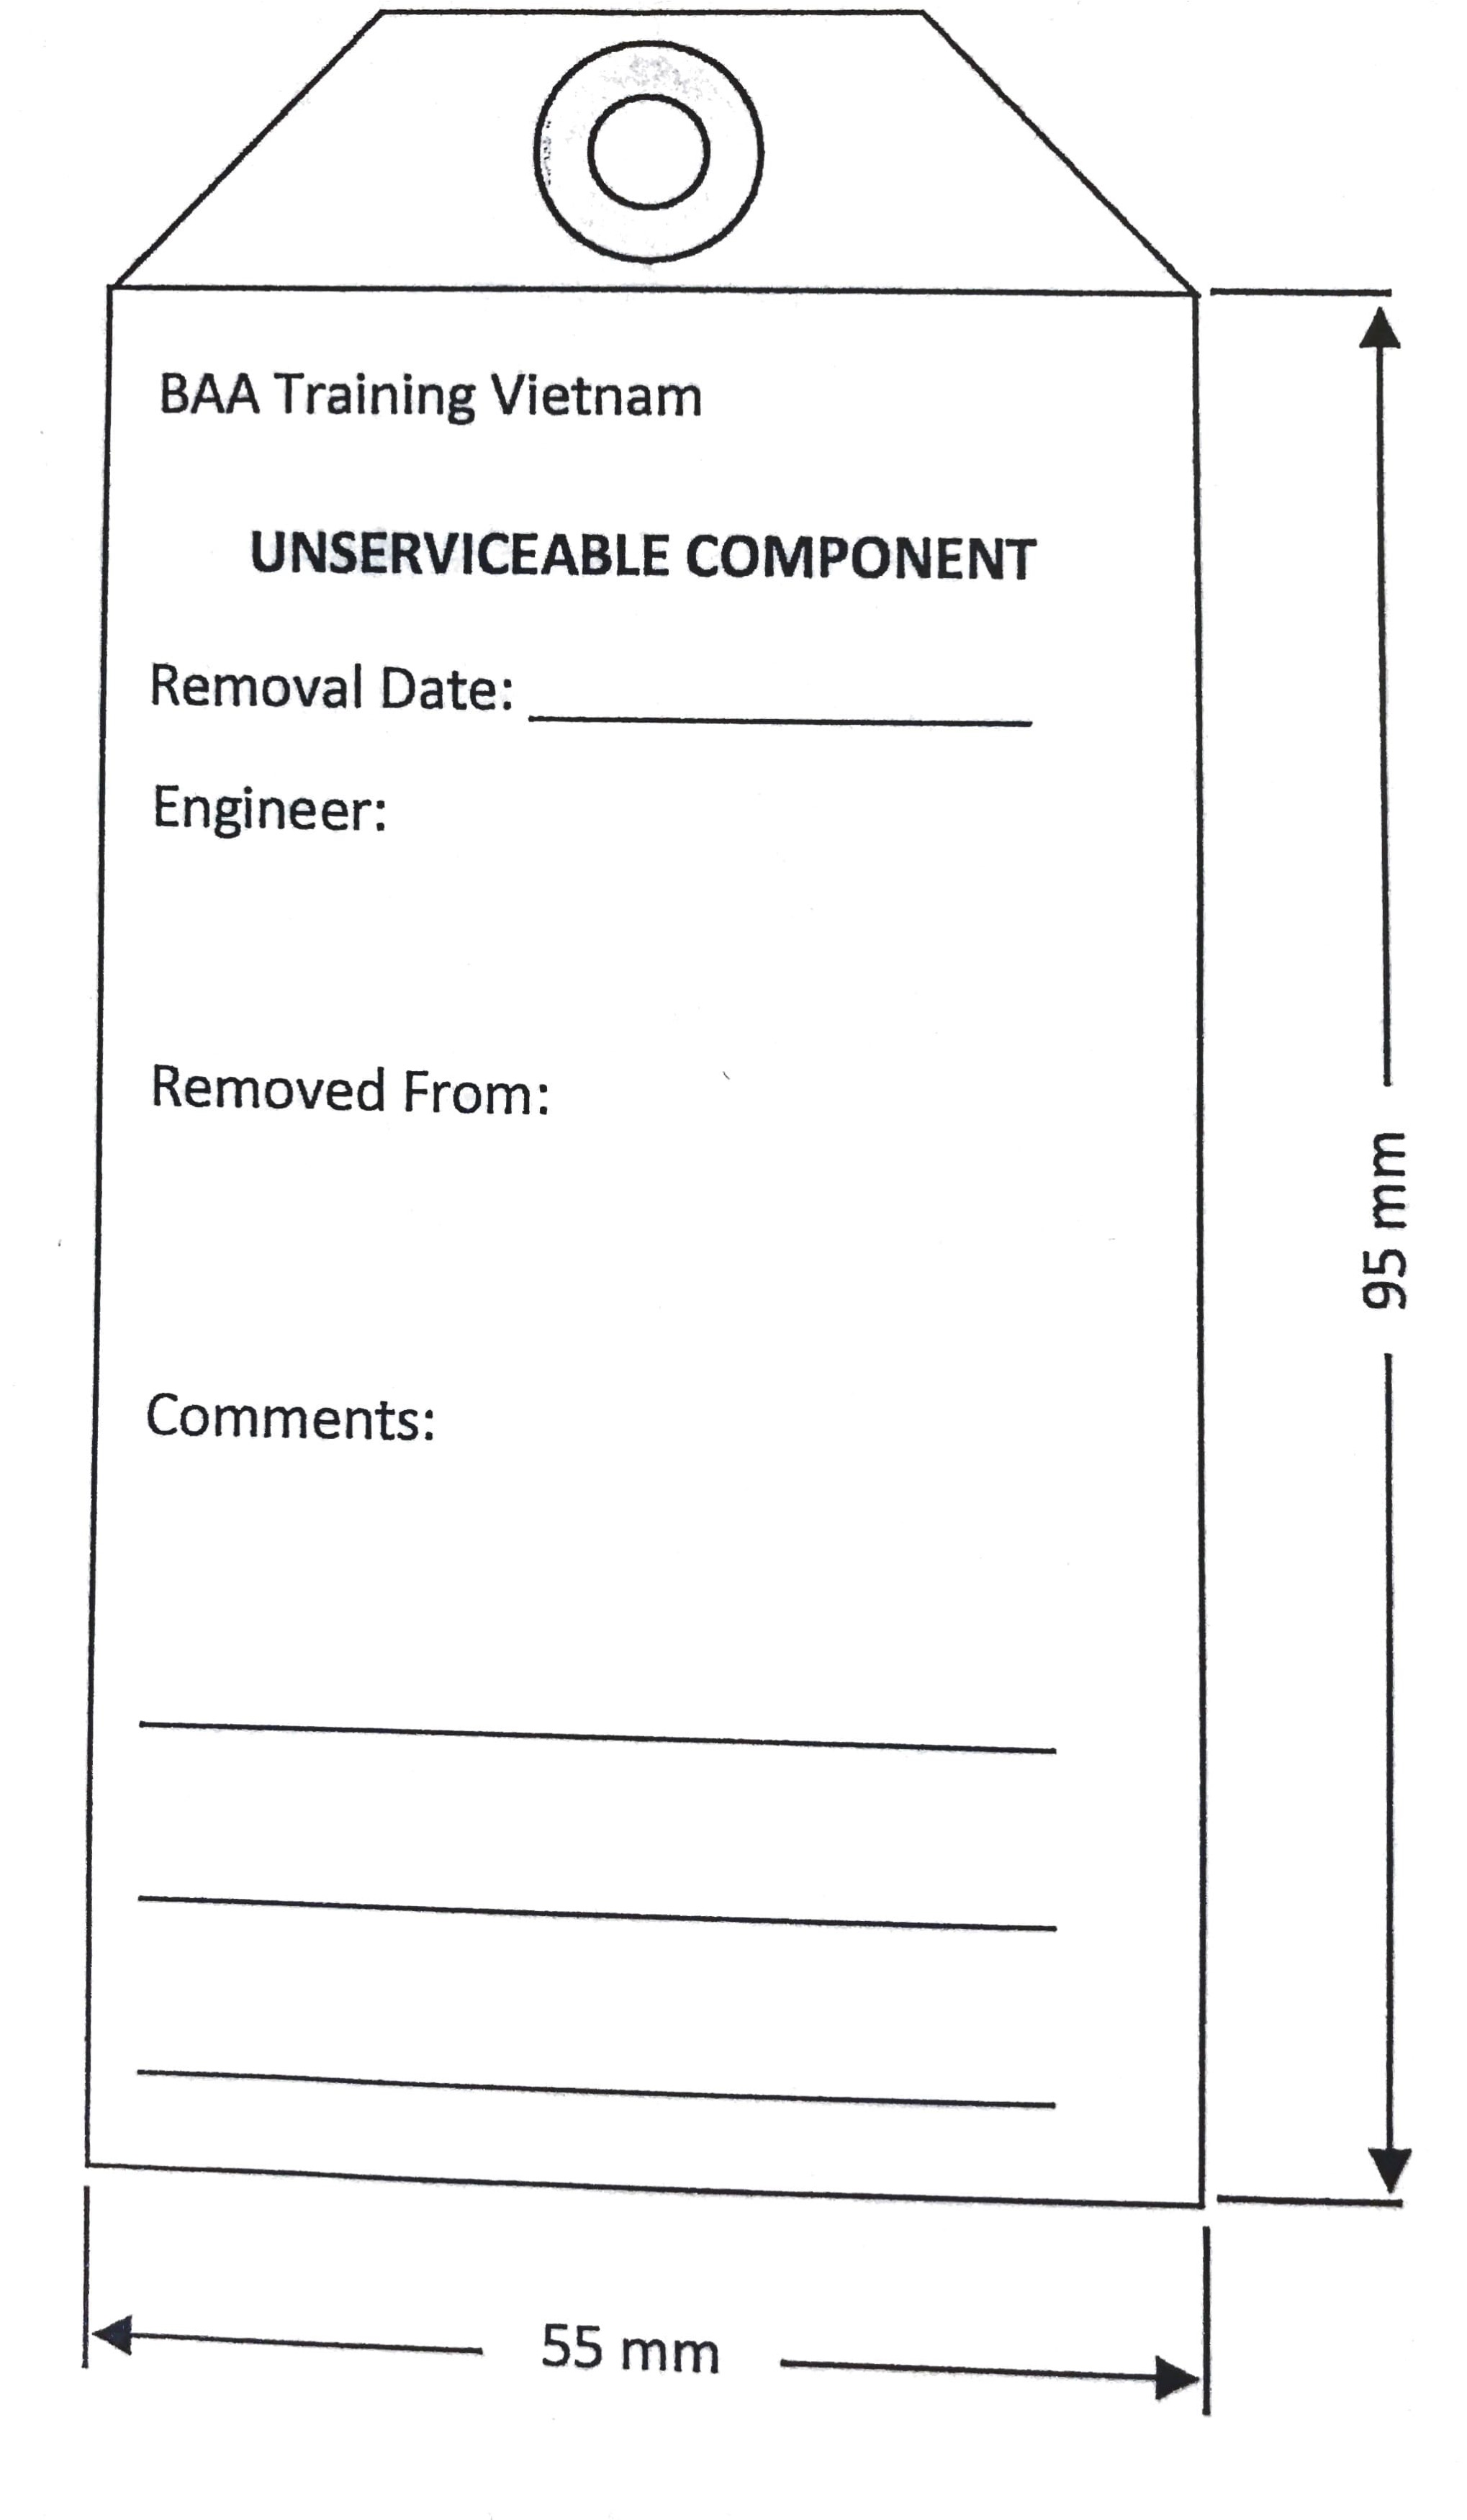
\includegraphics[width=0.6\linewidth]{img/label.JPG}
            \caption{Unserviceable Component label}
        \end{figure}
        The Unserviceable Component label should be filled according to the following guidance:
        \begin{itemize}
            \item \textbf{"Removal Date:"} - the date when component was removed;
            \item \textbf{"Engineer:"} - engineer name and signature who did remove the component;
            \item \textbf{"Removed From:"} - the place where the component was removed from;
            \item \textbf{"Comments:"} - any additional information to make easier recognition of unserviceable part. It is recommended to write here the No. of appropriate 
            Technical Defect Log.
        \end{itemize}
        Simulated aircraft components, for example Standby Altimeter, MCP Panel etc., shall be identified upon removal with a comment annotated "For Simulator Use Only". \\ 
        \vspace{3mm}
        All repairable unserviceable components dedicated to be sent to the simulator manufacturer, e.g. "Thales Training \& Simulation" (TT\&S), shall have the manufacturers 
        "Return for Repair Authorization" (RRA) form attached and their warranty status determined. 

    \subsection{Equipment Quality Check}
        After each training session simulator equipment condition should be checked for correct placing and any deterioration. Equipment Quality status and placement should be 
        reported using \textbf{Form 20 "Equipment Quality Check"}. \\ 
        \vspace{3mm}
        If technical defects are observed during Equipment Quality Check actions, then technical defects must be documented and managed by following the procedure "Unscheduled 
        Maintenance". \\ 
        \vspace{3mm}
        There are two checkbox options and adjacent comment field at each checklist item line.
        \begin{itemize}
            \item \textbf{"Yes"} - This should be checked if relevant equipment found placed in correct position and no defects are observed;
            \item \textbf{"No"} - This should be check if relevant equipment found not in dedicated position (e.g.Oxygen Mask is left on the floor). Actual place can be mentioned 
            in adjacent comment field for further crew behavior analysis.
        \end{itemize}
        If adjacent comment field is to small to fit desired comment description, then continuous Note number shoud be indicated there and actual comment text should be written 
        in general comment field below checklist table where notes numbering should be consistent as indicated along each checklist item. \\
        \vspace{3mm}
        Form usage explanation: 
        \begin{itemize}
            \item \textbf{Items 1.1 and 2.1:} equipment was found in dedicated positions and no defects were observed;
            \item \textbf{Item 1.2:} equipment was found in dedicated position and no defects were observed, however worn \textbf{Hygiene Pads} were renewed;
            \item \textbf{Item 1.3:} equipment was found not in dedicated position. Adjacent comment field was too short to accommodate desired comment text. Complete comment text 
            was referred as Note \#1 and written in general comments field below checklist items table;
            \item \textbf{Item 2.2:} equipment was found not in dedicated position and defect was observed. This defect was managed according procedure "Unscheduled Maintenance" and 
            related defect number was indicated in adjacent comments fields.
        \end{itemize}